%\documentclass[11pt]{jarticle}
\documentclass[a4paper,xelatex,ja=standard]{bxjsarticle}
\setlength{\textwidth}{7in}
\setlength{\textheight}{10in}
\setlength{\evensidemargin}{-0.25in}
\setlength{\oddsidemargin}{-0.25in}
\setlength{\topmargin}{-1in}

%\usepackage[dvipdfmx]{graphicx}
\usepackage{listings}

\title{情報科学II 第2回}

\date{2017年10月12日(木)}

\author{担当:高橋伸}

\begin{document}

\maketitle

\section{前回課題の解答例}

\begin{figure}[hbtp]
\begin{verbatim}
import processing.core.*;
public class ptest extends PApplet {
        public void settings() {
                size(500, 500);
        }
        public void setup() {
                background(0);
                ellipseMode(CORNER);
        }
        public void draw() {
                for (int i = 0; i < 12; i++) {
                        int x = (int) (250 + 100 * Math.cos(Math.toRadians(i * 30)));
                        int y = (int) (250 + 100 * Math.sin(Math.toRadians(i * 30)));
                        if (i % 2 == 0) {
                                ellipse(x, y, 10, 10);
                        } else {
                                rect(x, y, 10, 10);
                        }

                }
        }
        public static void main(String args[]) {
                PApplet.main("ptest");
        }
}
\end{verbatim}
\caption{前回の課題}
\label{kadai1}
\end{figure}

いろいろなプログラムが考えられるが,一つの解答例は図\ref{kadai1}の通りである.プログラム全体の構
成は,前回紹介したプログラムとほぼ同じである.つまり,ウインドウのサイズや色を setttings() と
setup() 内で記述している.実際に図形を描くプログラムは draw() 内に記述されている.

draw() 内のプログラムは for文を使って図形を繰り返し表示している.for文の中では,図形の座標位置を
まず計算し,それを x と y という変数に代入している.そして,その計算された座標位置に円か四角形を
描画している.円か四角形かのどちらを表示するかは,if文を使って場合分けしている.その場合分けの条
件は,変数 i を2で割った余りが 0 か 0 でないかによって場合分けをしている.余りが 0 であった場合
には,円が描かれる.また,そうでない場合には,四角が描かれる.変数 i は何番目に表示する図形かに
相当する番号で,0, 1, 2, ... と繰り返しの度に1づつ増えていく.従って,最初から 0番目は円,1番目
は四角,2番目は円,というように順番に表示されていく.

その他の補足的な説明は以下の通りである.
\begin{itemize}
  \item setup()内の,ellipseMode(CORNER) という命令は,ellipse()で指定した座標が円のどこの座標か?
    の設定を行う命令である.CORNER にすると,描画される円に外接する四角形の左上隅の座標が指定さ
    れた座標の位置だと解釈して描画されるようになる.
  \item Math.cos() や Math.sin() は,Math というパッケージの cos(),sin()メソッドであるということである.
  \item cos(), sin() の引数は角度であるが,単位としてはラジアンなので,「度」で指定したい場合に
    は変換する必要がある.Math.toRadians() という命令は「度」をラジアンに変換する命令である.
\end{itemize}

\section{メソッドの利用}


上記例でもそうであるが,プログラムの意味というのはそれほど明らかではない.そのため,1年後とかに
何のプログラムだか忘れてしまったら,改めてプログラムを読み直して理解しないといけないだろう.

また,もし同じ動作をプログラムの別の場所でもう一回実行したいという場合には,同じプログラムのかた
まりをコピーして書かないといけない.このコピーにはいくつもの弊害がある.まず,コピーして複数の場
所に同じ動作をするプログラムが存在しても,それらが同じであるということは,プログラム的には明示さ
れていないので,忘れられてしまう可能性がある.また,もし変更をしたいと思ったときに,全てのコピー
先をアップデートしないといけないが,これもエラーを引きおこしやすい.

そこで,一般のプログラミング言語では,プログラムのまとまりに名前をつけて再利用ができる仕組みが用
意されている.Java ではメソッド(method)がそれである.

例として,図\ref{method1}のプログラムを見てほしい.ここで,特に定義したメソッドは
matrixOfRectangles() と rowOfRectangles()である.18行目からのrowOfRectangles()は,横に四角形を並
べるように描画するというプログラムのかたまりに「rowOfRectangles」という名前を付けたものである.
このとき,さらに rowOfRectangles(float y) というように引数(ひきすう)がついている.これにより,こ
のメソッドを実行するときに,この値を使って位置を変えながら描画をすることができる.

また,12行目からの matrixOfRectangles()というメソッドは,四角形を行列状にならべるプログラ
ムであるが,ここで rowOfRectangles が使われている.このメソッドmatrixOfRectangles()では,
各行の縦位置を計算した値を変数yに代入し,それを rowOfRectangles()の引数として与えることで,
四角形の行が順番に上から下へ描画が行われるようなプログラムになっている.

プログラム全体としては,draw() の中に,matrixOfRectangles() と書かれているので,これが実行されて
マトリックスが表示される.なお, draw() や setup() やsettings() や main() は全てメソッドである.
これらのメソッドは,プログラムの実行後に,ある決められたタイミングで実行されることが決まっている.
当面は,draw() の中に書いたことが実行されて画面に表示されると考えておくと良い.このプログラムを
実行すると,図\ref{matrix}のような表示がされる.

\begin{figure}[hbtp]
%\lstset{numbers=left, numberstyle=\tiny, stepnumber=1, numbersep=5pt}
\lstset{numbers=left}
\begin{quote}
\begin{lstlisting}
import processing.core.*;
public class PTest2 extends PApplet{
        public void settings(){
                size(500,500);
        }
        public void setup(){
                background(0);
        }
        public void draw(){
                matrixOfRectangles();
        }
        public void matrixOfRectangles(){
                for(int j=0;j<10;j++){
                        int y = 100 + j * 10;
                        rowOfRectangles(y);
                }
        }
        public void rowOfRectangles(int y){
                for(int i=0; i<10; i++){
                        int x = 100 + i * 10;
                        rect(x, y, 10, 10);      
                }
        }
        public static void main(String args[]) {
            PApplet.main("PTest2");
        }
}
\end{lstlisting}
\end{quote}
\caption{メソッドの例}
\label{method1}
\end{figure}
\begin{figure}[hbtp]
\centerline{
 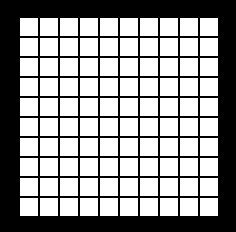
\includegraphics[scale=1.0]{matrix.png}
}
\caption{マトリックス}
\label{matrix}
\end{figure}


\section{課題}

\subsection{課題1}
上で説明した四角形を並べるプログラムをmatrixOfRectangles()とrowOfRectangles()というメソッドを使
わないプログラムに改造してみよう.つまり,改造されたプログラムでは,draw()メソッドの中にマトリッ
クスを描画するプログラム部分がすべて展開されて記述されているようなプログラムになる.なお,動作
(描画)結果はもとのプログラムと変更がないものとする.

\subsection{課題2}
ロボットのようなものを描画をするメソッドを定義し,それを使ってロボットを画面にたくさん描画するプ
ログラムを作れ.個々のロボットの形は自由であるので好きな形にして良い.(例:図\ref{kadai2})

\begin{figure}[hbtp]
\centerline{
 
\includegraphics[scale=1.0]{robots.png}
}
\caption{ロボットのようなもの}
\label{kadai2}
\end{figure}



\end{document}




